\section{Numerical Mathematics Fundamendals}

\subsection{Problem 4.8}

\begin{figure}[!ht]
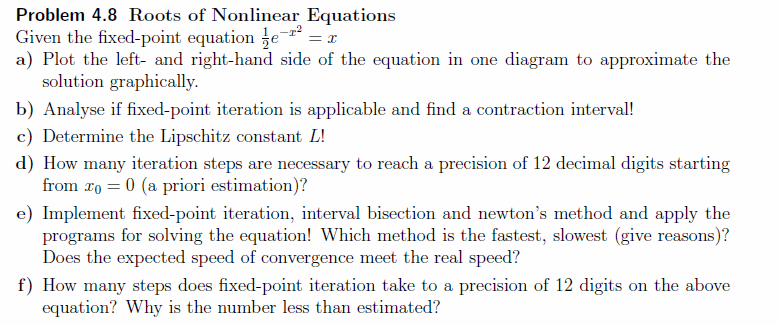
\includegraphics[width=1\textwidth]{chapters/images/desc-4-8}
\end{figure}

First the function needs to be defined. The're are two ways to find a root, setting function equal to 0 and setting the function equal to $x$. The function which is to be set equal to 0 is going to be called $f(x)$, while the function to be set equal to $x$ is going to be called $fFixed(x)$, with their derived functions $fDerived(x)$ and $fFixedDerived(x)$ respectively:

\begin{lstlisting}[caption=Different functions for the equation]
def fFixed(x):
	return 0.5 * pow(math.e, -pow(x, 2));

def fFixedDerived(x):
	return -pow(math.e, -pow(x, 2)) * x;

def f(x):
	return fFixed(x) - x;

def fDerived(x):
	return fFixedDerived(x) - 1;
\end{lstlisting}

These functions will be used in the code of the following subtasks, where method to find a root determines which of them is going to be used.


\subsubsection{a)}

With the following code both sides of the equation will be plotted:

\begin{lstlisting}[caption=Problem 4.8 a)]
xses = [];
fLeft = [];
fRight = [];

for i in range(200):
	x = (i / 100.0) - 1;
	
	xses.append(x);
	fLeft.append(fFixed(x));
	fRight.append(x);

plt.plot(xses, fLeft);
plt.plot(xses, fRight);
plt.xlabel('x');
plt.ylabel('y');
plt.show();
\end{lstlisting}

The resulting plot of both sides of the equation looks like the following:

\begin{figure}[!ht]
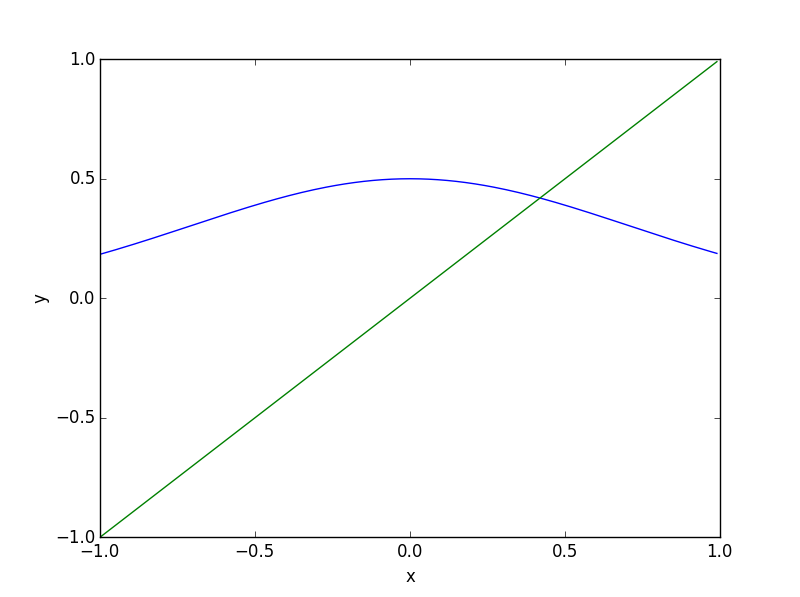
\includegraphics[width=1\textwidth]{chapters/images/figure-4-8-a}
\caption{Graphical solution for the root}
\end{figure}

The approximate solution can be found graphically by looking for an intersection of both functions. The functions intersect close to the point $(0.45~|~0.45)$, therefore the root of the function is approximately 0.45.


\subsubsection{b)}

To use the fixed point interation method for finding a root of a function within an interval $[a, b] \rightarrow [a, b]$, the function has to be a contraction within this interval. A function is a contraction if the Lipschitz constant $L$ is greater than $0$ and smaller than $1$. Within the interval $[0, 1] \rightarrow [0, 1]$, where we graphically estimated the root in the sub task a), the Lipschitz constant is about $0.4289$ (see sub task c)), therefore the condition holds and fixed point interation is applicable.

\subsubsection{c)}

The Lipschitz constant is the highest increase or decrease of a function, or in other words the maximum of the absolute value of the minimum and maximum of the first derivative of said function.
The second derivative of the function has two roots, at $x_1 = -0.70711$ and $x_2 = 0.70711$. These are the maxima and minima of the first derivative, and therefore the highest increase of the function and the Lipschitz constant $L$. Since only $x_2$ is in the contraction interval, the Lipschitz constant can simply be calculated by plugging it into the function $f$.

\begin{lstlisting}[caption=Problem 4.8 c)]
# -0.70711 and 0.70711 are roots of the 2nd derivative of f
lipschitz = abs(fFixedDerived(0.70711));

print("L = " + str(lipschitz));
\end{lstlisting}

The resulting $L$ is:

\begin{lstlisting}[caption=Result of 4.8 c), keywordstyle=\color{black}]
L = 0.428881942471
\end{lstlisting}

\subsubsection{d)}

With the Lipschitz constant from c), the maximum number of iterations required to find a root with a given precision by using the fixed point iteration method can be calculated with the a priori estimation:

\begin{lstlisting}[caption=Problem 4.8 d)]
steps = 0;
err = 1;
xdiff = f(0);

while err > 1e-12:
	steps = steps + 1;
	err = (pow(lipschitz, steps) / (1 - lipschitz)) * xdiff;

print(str(steps) + " iteration steps required");
\end{lstlisting}

The result of this estimation is:

\begin{lstlisting}[caption=Result of 4.8 d), keywordstyle=\color{black}]
33 iteration steps required
\end{lstlisting}

Therefore, to get a precision of 12 decimal digits for our function $f$ a maximum of 33 iterations are needed.

\subsubsection{e)}

First we need a function to see whether our calculated value is precise enough:

\begin{lstlisting}[caption=Determine if an approximation is precise enough]
def isPreciseEnough(val, goal, precision):
	f = pow(10, precision);

	return math.floor(val * f) == math.floor(goal * f);
\end{lstlisting}

The implementation of fixed point iteration could be realized in the following way:

\begin{lstlisting}[caption=Fixed point iteration method]
def getFixedPoint(x0, goal, precision):
	x = x0;
	steps = 1;
	
	while steps < 100:
		x = fFixed(x);
		
		if (isPreciseEnough(x, goal, precision)):
			break;
		
		steps = steps + 1;
	
	return steps;
\end{lstlisting}

The interval bisection method can be implemented like this:

\begin{lstlisting}[caption=Interval Bisection method]
def mySign(x):
	return -1 if x < 0 else 1;

def getRootBisection(pXA, pXB, goal, precision):
	xa = pXA;
	xb = pXB;
	xm = -1;
	steps = 1;
	
	while steps < 100:
		xm = xa + (xb - xa) / 2.0;
		
		if (isPreciseEnough(xm, goal, precision)):
			break;
		
		if mySign(f(xa)) != mySign(f(xm)):
			xb = xm;
		else:
			xa = xm;
		
		steps = steps + 1;
	
	return steps;
\end{lstlisting}

Finally a function to approximate the root of a function with Newton's method could be realized the following way:

\begin{lstlisting}[caption=Newton's method]
def getRootNewton(x0, goal, precision):
	x = x0;
	steps = 1;
	
	while steps < 100:
		fD = fDerived(x);
		
		if abs(fD) < 0.00001: fD = 0.00001;
		
		x = x - float(f(x) / float(fD));
		
		if (isPreciseEnough(x, goal, precision)):
			break;
		
		steps = steps + 1;
	
	return steps;
\end{lstlisting}

Afterwards, the three methods can be compared regarding how much time is needed to find the root of the function with the desired precision.

\begin{lstlisting}[caption=Testing the three methods]
def getTime():
	return time.time();

def printTimeDiff(startTime, endTime):
	averageMS = round((endTime - startTime) / 10.0, 5);
	print("average time taken: " + str(averageMS) + " milliseconds");

def findRoot(type, goal, precision, p1 = 0, p2 = 0):
	startTime = getTime();
	
	steps = 0;
	
	for i in range(10000):
		param1 = p1 + 0.000001 * math.sin(i * 7);
	
		if (type == 0): steps = getFixedPoint(param1, goal, precision);
		elif (type == 1): steps = getRootBisection(param1, p2, goal, precision);
		else: steps = getRootNewton(param1, goal, precision);
	
	print("steps taken: " + str(steps));
	printTimeDiff(startTime, getTime());

def getFixedPointRec2(x, maxSteps, stepsTaken):
	newX = fFixed(x);
	
	if stepsTaken < maxSteps:
		return getFixedPointRec2(newX, maxSteps, stepsTaken + 1);
	else:
		return newX;

def getFixedPointRec1(x0, maxSteps):
	return getFixedPointRec2(x0, maxSteps, 1);

# get a precise enough approximation of the root 
fP33 = getFixedPointRec1(0, 100);

precision = 6;
print("correct digits required: " + str(precision));

print("fixed point iteration:");
findRoot(0, fP33, precision, 0, -1);

print("interval bisection:");
findRoot(1, fP33, precision, 0, 1);

print("newton's method:");
findRoot(2, fP33, precision, 0, -1);

precision = 12;
print("correct digits required: " + str(precision));

print("fixed point iteration:");
findRoot(0, fP33, precision, 0, -1);

print("interval bisection:");
findRoot(1, fP33, precision, 0, 1);

print("newtons method:");
findRoot(2, fP33, precision, 0, -1);

precision = 18;
print("correct digits required: " + str(precision));

print("fixed point iteration:");
findRoot(0, fP33, precision, 0, -1);

print("interval bisection:");
findRoot(1, fP33, precision, 0, 1);

print("newtons method:");
findRoot(2, fP33, precision, 0, -1);
\end{lstlisting}

The results of the tests are the following:

\begin{lstlisting}[caption=Result of 4.8 e), keywordstyle=\color{black}]
correct digits required: 6
fixed point iteration:
steps taken: 14
average time taken: 0.0382 milliseconds

interval bisection:
steps taken: 17
average time taken: 0.0914 milliseconds

newtons method:
steps taken: 4
average time taken: 0.0237 milliseconds

correct digits required: 12
fixed point iteration:
steps taken: 27
average time taken: 0.1185 milliseconds

interval bisection:
steps taken: 40
average time taken: 0.2703 milliseconds

newtons method:
steps taken: 4
average time taken: 0.0321 milliseconds

correct digits required: 18
fixed point iteration:
steps taken: 35
average time taken: 0.1501 milliseconds

interval bisection:
steps taken: 51
average time taken: 0.3547 milliseconds

newtons method:
steps taken: 5
average time taken: 0.0377 milliseconds
\end{lstlisting}

As seen Newton's method is much faster than the other two methods, with up to almost a tenth of computational time. The second fastest method is fixed point iteration, while the interval bisection method is the slowest.

The reason why Newton's method is the fastest is because it also utilizes the first derivative of the function, which is a valuable information to find the root quicker. Interval bisection is the slowest method because it doesn't even use the function value unlike fixed point iteration. Instead, the interval is halved halved with each step, no matter how close one bound is to the root of the function (except when the approximation is already precise enough of course).


\subsubsection{f)}

To get a precise enough approximation of the root, 27 steps were needed instead of the estimated 33 steps in d). The reason it took less iterations is because the a priori estimation always asumes the worst case scenario.

